% !TeX program = pdflatex
\documentclass[11pt,a4paper]{article}
\input{preamble}
\usepackage[margin=2.2cm]{geometry}
\usepackage{tikz}
\setlength{\parindent}{0pt}
\setlength{\parskip}{7pt}
\begin{document}
{\small\sffamily\color{teal} {{TITLE}}}\par\hrule\medskip
\section*{IELTS Writing practice bank}
\textit{Đề luyện tự biên soạn; số liệu giả định.}\par
\tableofcontents
\clearpage
\phantomsection
\addcontentsline{toc}{section}{Line graph}
\section*{WRITING TASK 1}
You should spend about 20 minutes on this task.

\begin{quote}\large The line graph shows the average number of daily visits to three public libraries in the fictional city of Bellford between 2010 and 2025.
\end{quote}
Describe the main features of the information, select relevant details, and make comparisons where appropriate.

\begin{center}
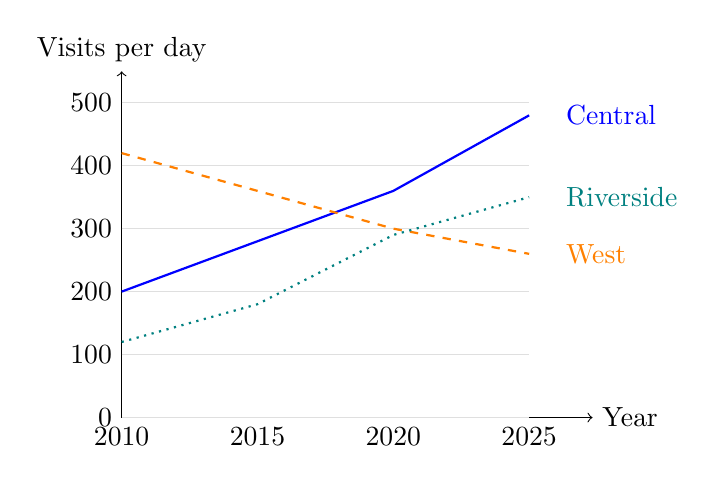
\begin{tikzpicture}[x=0.115cm,y=0.008cm]
\draw[->] (0,0)--(52,0) node[right]{Year}; \draw[->] (0,0)--(0,550) node[above]{Visits per day};
\foreach \v in {0,100,200,300,400,500}{\draw[gray!25] (0,\v)--(45,\v);\node[left] at (0,\v){\v};}
\foreach \x/\v in {0/2010,15/2015,30/2020,45/2025}{\node[below] at (\x,0){\v};}
\draw[blue,thick] (0,200)--(15,280)--(30,360)--(45,480);
\draw[orange,thick,dashed] (0,420)--(15,360)--(30,300)--(45,260);
\draw[teal,thick,dotted] (0,120)--(15,180)--(30,290)--(45,350);
\node[blue,anchor=west] at (48,480){Central};\node[orange,anchor=west] at (48,260){West};\node[teal,anchor=west] at (48,350){Riverside};
\end{tikzpicture}
\end{center}
Write at least 150 words.
\par\bigskip
{\footnotesize\color{gray} Original practice material; fictional settings and data. Not an official IELTS examination paper.}

\clearpage
\phantomsection
\addcontentsline{toc}{section}{Bar chart}
\section*{WRITING TASK 1}
You should spend about 20 minutes on this task.

\begin{quote}\large The bar chart compares the percentages of commuters using four main forms of transport in Bellford in 2005 and 2025.
\end{quote}
Describe the main features of the information, select relevant details, and make comparisons where appropriate.

\begin{center}
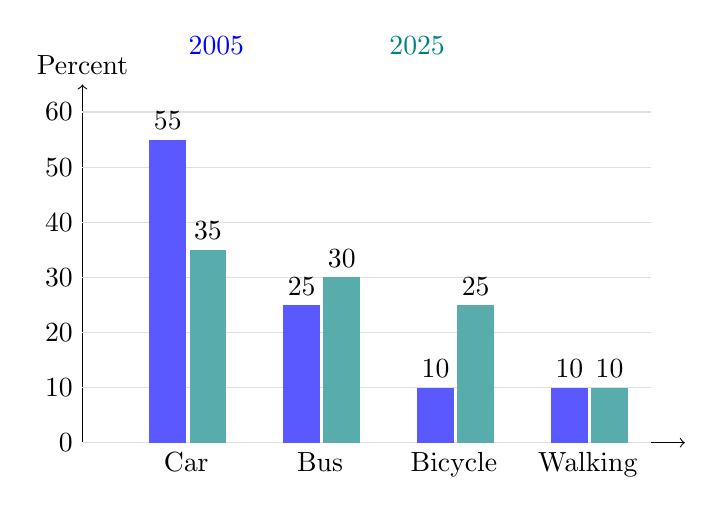
\begin{tikzpicture}[x=0.85cm,y=0.07cm]
\draw[->] (0,0)--(9,0);\draw[->] (0,0)--(0,65) node[above]{Percent};
\foreach \v in {0,10,20,30,40,50,60}{\draw[gray!25] (0,\v)--(8.5,\v);\node[left] at (0,\v){\v};}
\foreach \x/\a/\b/\name in {1/55/35/Car,3/25/30/Bus,5/10/25/Bicycle,7/10/10/Walking}{
\fill[blue!65] (\x,0) rectangle +(0.55,\a);\fill[teal!65] (\x+0.6,0) rectangle +(0.55,\b);
\node[above] at (\x+0.275,\a){\a};\node[above] at (\x+0.875,\b){\b};\node[below] at (\x+0.55,0){\name};}
\node[blue] at (2,72){2005};\node[teal] at (5,72){2025};
\end{tikzpicture}
\end{center}
Write at least 150 words.
\par\bigskip
{\footnotesize\color{gray} Original practice material; fictional settings and data. Not an official IELTS examination paper.}

\clearpage
\phantomsection
\addcontentsline{toc}{section}{Pie chart}
\section*{WRITING TASK 1}
You should spend about 20 minutes on this task.

\begin{quote}\large The pie charts show how household energy use was distributed among four purposes in a fictional country in 2000 and 2025.
\end{quote}
Describe the main features of the information, select relevant details, and make comparisons where appropriate.

\begin{center}
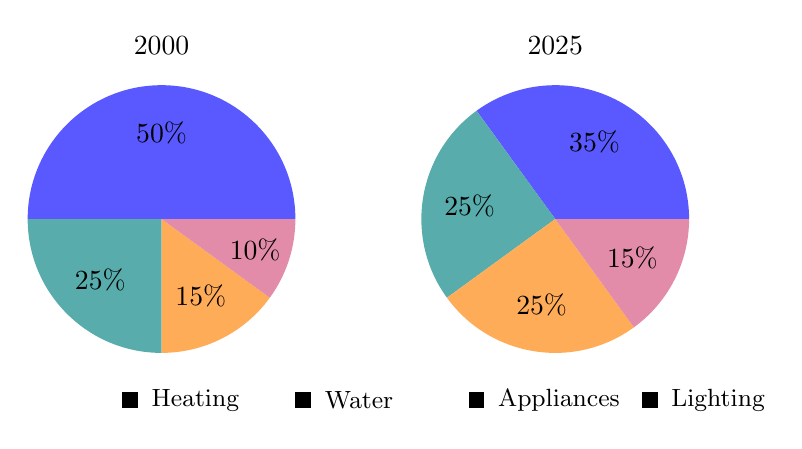
\begin{tikzpicture}
\begin{scope}[shift={(0,0)}]
\fill[blue!65] (0,0)--(0:1.7) arc (0:180:1.7)--cycle;
\fill[teal!65] (0,0)--(180:1.7) arc (180:270:1.7)--cycle;
\fill[orange!65] (0,0)--(270:1.7) arc (270:324:1.7)--cycle;
\fill[purple!45] (0,0)--(324:1.7) arc (324:360:1.7)--cycle;
\node at (0,2.2){2000};\node at (90:1.1){50\%};\node at (225:1.1){25\%};\node at (297:1.1){15\%};\node at (342:1.25){10\%};
\end{scope}
\begin{scope}[shift={(5,0)}]
\fill[blue!65] (0,0)--(0:1.7) arc (0:126:1.7)--cycle;
\fill[teal!65] (0,0)--(126:1.7) arc (126:216:1.7)--cycle;
\fill[orange!65] (0,0)--(216:1.7) arc (216:306:1.7)--cycle;
\fill[purple!45] (0,0)--(306:1.7) arc (306:360:1.7)--cycle;
\node at (0,2.2){2025};\node at (63:1.1){35\%};\node at (171:1.1){25\%};\node at (261:1.1){25\%};\node at (333:1.1){15\%};
\end{scope}
\foreach \x/\color/\name in {-0.5/blue/Heating,1.7/teal/Water,3.9/orange/Appliances,6.1/purple/Lighting}{\fill[\color!65] (\x,-2.4) rectangle +(0.2,0.2);\node[anchor=west,font=\small] at (\x+0.25,-2.3){\name};}
\end{tikzpicture}
\end{center}
Write at least 150 words.
\par\bigskip
{\footnotesize\color{gray} Original practice material; fictional settings and data. Not an official IELTS examination paper.}

\clearpage
\phantomsection
\addcontentsline{toc}{section}{Table}
\section*{WRITING TASK 1}
You should spend about 20 minutes on this task.

\begin{quote}\large The table gives enrolment and completion figures for four community education courses in Bellford in 2024.
\end{quote}
Describe the main features of the information, select relevant details, and make comparisons where appropriate.

\begin{center}
\renewcommand{\arraystretch}{1.6}
\begin{tabular}{|l|r|r|r|}\hline
Course & Enrolled students & Completed students & Fee (USD)\\\hline
Languages & 240 & 204 & 120\\
Computing & 180 & 162 & 150\\
Cooking & 150 & 135 & 90\\
Photography & 100 & 70 & 180\\\hline
\end{tabular}
\end{center}
Write at least 150 words.
\par\bigskip
{\footnotesize\color{gray} Original practice material; fictional settings and data. Not an official IELTS examination paper.}

\clearpage
\phantomsection
\addcontentsline{toc}{section}{Mixed / multiple visuals}
\section*{WRITING TASK 1}
You should spend about 20 minutes on this task.

\begin{quote}\large The chart shows the numbers of visitors to three museums in 2024. The table gives their average spending per visit in the same year.
\end{quote}
Describe the main features of the information, select relevant details, and make comparisons where appropriate.

\begin{center}
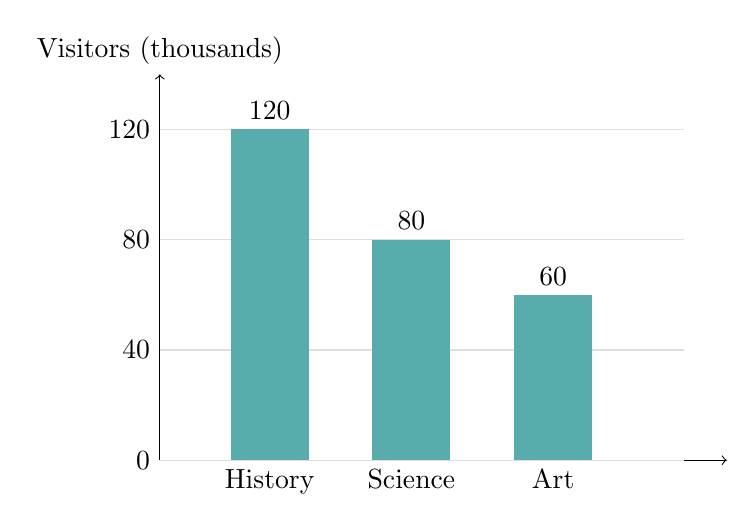
\begin{tikzpicture}[x=1.8cm,y=0.035cm]
\draw[->] (0,0)--(4,0);\draw[->] (0,0)--(0,140) node[above]{Visitors (thousands)};
\foreach \v in {0,40,80,120}{\node[left] at (0,\v){\v};\draw[gray!25] (0,\v)--(3.7,\v);}
\foreach \x/\v/\name in {0.5/120/History,1.5/80/Science,2.5/60/Art}{\fill[teal!65] (\x,0) rectangle +(0.55,\v);\node[above] at (\x+0.275,\v){\v};\node[below] at (\x+0.275,0){\name};}
\end{tikzpicture}
\par\bigskip\begin{tabular}{|l|r|}\hline Museum & Spending per visitor (USD)\\\hline History & 8\\Science & 15\\Art & 20\\\hline\end{tabular}
\end{center}
Write at least 150 words.
\par\bigskip
{\footnotesize\color{gray} Original practice material; fictional settings and data. Not an official IELTS examination paper.}

\clearpage
\phantomsection
\addcontentsline{toc}{section}{Process / cycle}
\section*{WRITING TASK 1}
You should spend about 20 minutes on this task.

\begin{quote}\large The diagram illustrates how rainwater is collected and prepared for non-drinking uses in a residential building.
\end{quote}
Describe the main features of the information, select relevant details, and make comparisons where appropriate.

\begin{center}
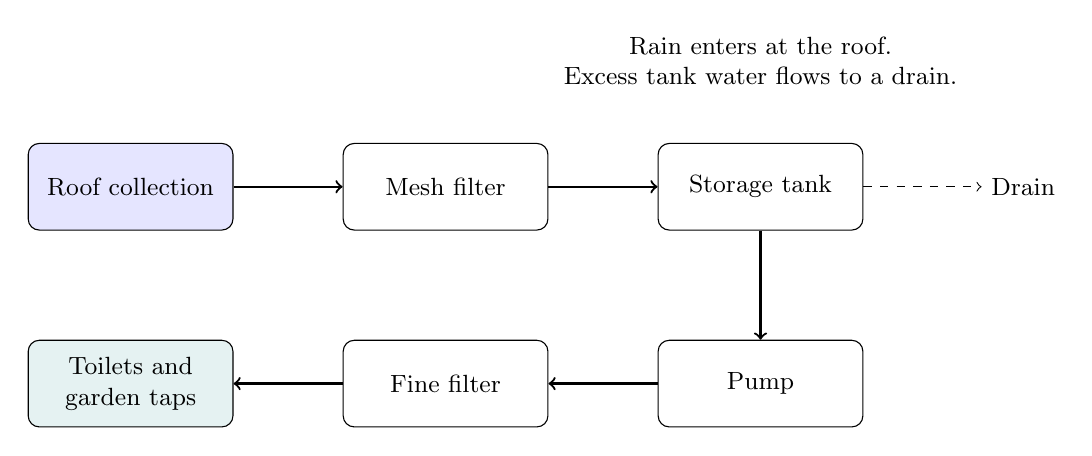
\begin{tikzpicture}[every node/.style={font=\small},box/.style={draw,rounded corners,align=center,minimum width=2.6cm,minimum height=1.1cm}]
\node[box,fill=blue!10] (a) at (0,0){Roof collection};\node[box] (b) at (4,0){Mesh filter};\node[box] (c) at (8,0){Storage tank};
\node[box] (d) at (8,-2.5){Pump};\node[box] (e) at (4,-2.5){Fine filter};\node[box,fill=teal!10] (f) at (0,-2.5){Toilets and\\garden taps};
\draw[->,thick] (a)--(b);\draw[->,thick] (b)--(c);\draw[->,thick] (c)--(d);\draw[->,thick] (d)--(e);\draw[->,thick] (e)--(f);
\node[font=\small,align=center] at (8,1.6){Rain enters at the roof.\\Excess tank water flows to a drain.};\draw[->,dashed] (c.east)--+(1.5,0) node[right]{Drain};
\end{tikzpicture}
\end{center}
Write at least 150 words.
\par\bigskip
{\footnotesize\color{gray} Original practice material; fictional settings and data. Not an official IELTS examination paper.}

\clearpage
\phantomsection
\addcontentsline{toc}{section}{Map / plan}
\section*{WRITING TASK 1}
You should spend about 20 minutes on this task.

\begin{quote}\large The plans show a neighbourhood square in Bellford in 2000 and after redevelopment in 2025.
\end{quote}
Describe the main features of the information, select relevant details, and make comparisons where appropriate.

\begin{center}
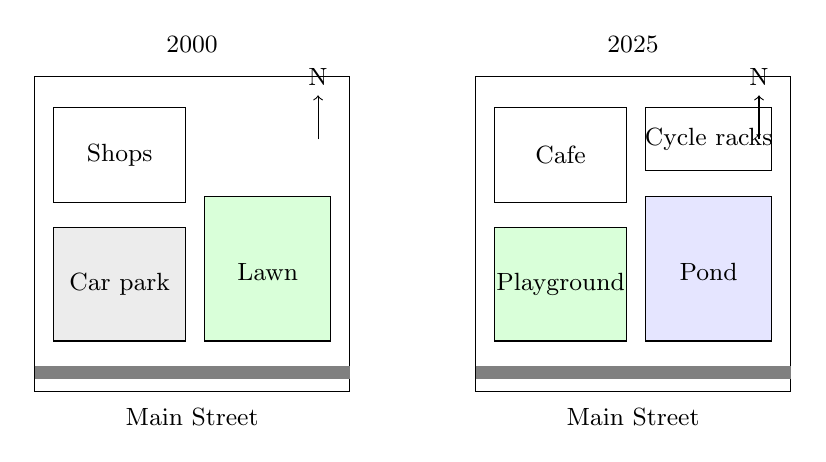
\begin{tikzpicture}[x=0.8cm,y=0.8cm,every node/.style={font=\small,align=center}]
\foreach \x/\year in {0/2000,7/2025}{\draw (\x,0) rectangle +(5,5);\node at (\x+2.5,5.5){\year};\draw[gray,line width=5pt] (\x,0.3)--+(5,0);\node at (\x+2.5,-0.4){Main Street};\draw[->] (\x+4.5,4)--+(0,0.7) node[above]{N};}
\draw[fill=gray!15] (0.3,0.8) rectangle (2.4,2.6);\node at (1.35,1.7){Car park};
\draw[fill=green!15] (2.7,0.8) rectangle (4.7,3.1);\node at (3.7,1.9){Lawn};
\draw (0.3,3) rectangle (2.4,4.5);\node at (1.35,3.75){Shops};
\draw[fill=green!15] (7.3,0.8) rectangle (9.4,2.6);\node at (8.35,1.7){Playground};
\draw[fill=blue!10] (9.7,0.8) rectangle (11.7,3.1);\node at (10.7,1.9){Pond};
\draw (7.3,3) rectangle (9.4,4.5);\node at (8.35,3.75){Cafe};\draw (9.7,3.5) rectangle (11.7,4.5);\node at (10.7,4){Cycle racks};
\end{tikzpicture}
\end{center}
Write at least 150 words.
\par\bigskip
{\footnotesize\color{gray} Original practice material; fictional settings and data. Not an official IELTS examination paper.}

\clearpage
\phantomsection
\addcontentsline{toc}{section}{Object / system diagram}
\section*{WRITING TASK 1}
You should spend about 20 minutes on this task.

\begin{quote}\large The diagram shows the main components of a solar-powered ventilation unit and how air moves through it.
\end{quote}
Describe the main features of the information, select relevant details, and make comparisons where appropriate.

\begin{center}
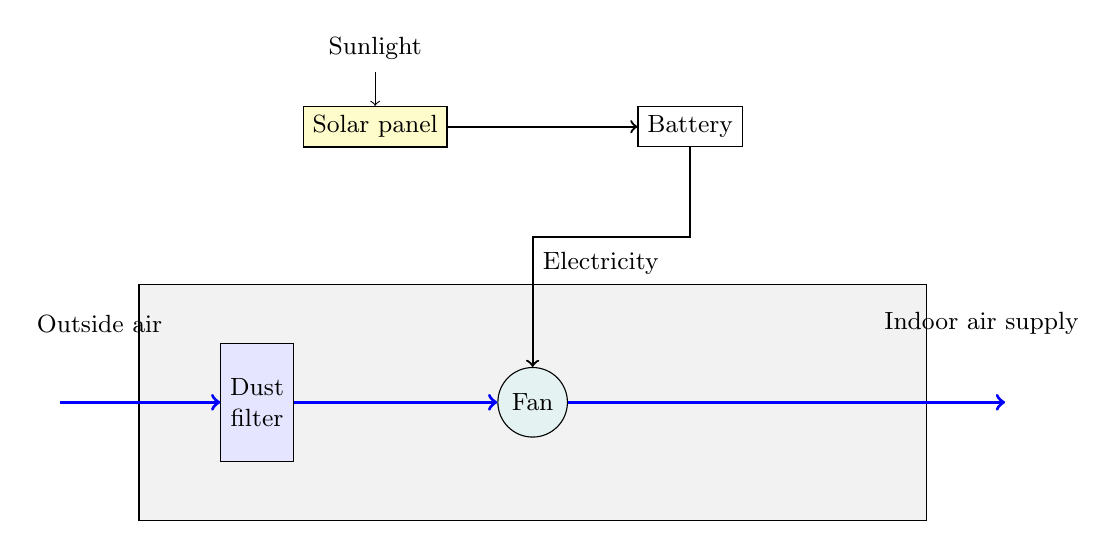
\begin{tikzpicture}[every node/.style={font=\small,align=center}]
\draw[fill=gray!10] (0,0) rectangle (10,3);
\node[draw,fill=blue!10,minimum height=1.5cm] (filter) at (1.5,1.5){Dust\\filter};
\node[draw,circle,fill=teal!10] (fan) at (5,1.5){Fan};
\draw[->,very thick,blue] (-1,1.5)--(filter);\node at (-0.5,2.5){Outside air};
\draw[->,very thick,blue] (filter)--(fan);\draw[->,very thick,blue] (fan)--(11,1.5);\node at (10.7,2.5){Indoor air supply};
\node[draw,fill=yellow!20] (solar) at (3,5){Solar panel};\node[draw] (battery) at (7,5){Battery};
\draw[->,thick] (solar)--(battery);\draw[->,thick] (battery)--(7,3.6)--(5,3.6)--(fan) node[pos=0.2,right]{Electricity};
\node at (3,6){Sunlight};\draw[->] (3,5.7)--(solar);
\end{tikzpicture}
\end{center}
Write at least 150 words.
\par\bigskip
{\footnotesize\color{gray} Original practice material; fictional settings and data. Not an official IELTS examination paper.}

\clearpage
\phantomsection
\addcontentsline{toc}{section}{Formal letter}
\section*{WRITING TASK 1}
You should spend about 20 minutes on this task.

\begin{quote}\large You attend an evening study group at a public library. The library plans to close earlier, which would affect your group. Write a letter to the library manager. In your letter:
\begin{itemize}
\item explain how your group uses the library
\item describe the difficulty the new hours would cause
\item suggest a practical alternative
\end{itemize}
\end{quote}
You do not need to write any addresses.

Write at least 150 words.
\par\bigskip
{\footnotesize\color{gray} Original practice material; fictional settings and data. Not an official IELTS examination paper.}

\clearpage
\phantomsection
\addcontentsline{toc}{section}{Semi-formal letter}
\section*{WRITING TASK 1}
You should spend about 20 minutes on this task.

\begin{quote}\large You work part-time in a local bookshop and know the owner well. You need to change your working hours for the next month. Write a letter to the owner. In your letter:
\begin{itemize}
\item explain why you need different hours
\item suggest a new schedule
\item describe how you could help avoid disruption
\end{itemize}
\end{quote}
You do not need to write any addresses.

Write at least 150 words.
\par\bigskip
{\footnotesize\color{gray} Original practice material; fictional settings and data. Not an official IELTS examination paper.}

\clearpage
\phantomsection
\addcontentsline{toc}{section}{Informal letter}
\section*{WRITING TASK 1}
You should spend about 20 minutes on this task.

\begin{quote}\large A friend from another town has asked about visiting you for a weekend. Write a letter to your friend. In your letter:
\begin{itemize}
\item suggest a suitable weekend
\item describe two activities you could do together
\item explain how your friend can reach your home
\end{itemize}
\end{quote}
You do not need to write any addresses.

Write at least 150 words.
\par\bigskip
{\footnotesize\color{gray} Original practice material; fictional settings and data. Not an official IELTS examination paper.}

\clearpage
\phantomsection
\addcontentsline{toc}{section}{Opinion / agree--disagree}
\section*{WRITING TASK 2}
You should spend about 40 minutes on this task.

\begin{quote}\large Secondary schools should teach students how to repair everyday household items, even if this reduces the time available for other subjects. To what extent do you agree or disagree?
\end{quote}
Support your ideas with reasons and relevant examples.

Write at least 250 words.
\par\bigskip
{\footnotesize\color{gray} Original practice material; fictional settings and data. Not an official IELTS examination paper.}

\clearpage
\phantomsection
\addcontentsline{toc}{section}{Discuss both views (+ opinion)}
\section*{WRITING TASK 2}
You should spend about 40 minutes on this task.

\begin{quote}\large Some people believe public libraries should spend most of their budget on digital resources. Others think printed books and physical reading spaces should remain the priority. Discuss both views and give your own opinion.
\end{quote}
Support your ideas with reasons and relevant examples.

Write at least 250 words.
\par\bigskip
{\footnotesize\color{gray} Original practice material; fictional settings and data. Not an official IELTS examination paper.}

\clearpage
\phantomsection
\addcontentsline{toc}{section}{Advantages \& disadvantages}
\section*{WRITING TASK 2}
You should spend about 40 minutes on this task.

\begin{quote}\large An increasing number of towns are closing central streets to traffic at weekends so that local markets can take place. What are the advantages and disadvantages of this approach?
\end{quote}
Support your ideas with reasons and relevant examples.

Write at least 250 words.
\par\bigskip
{\footnotesize\color{gray} Original practice material; fictional settings and data. Not an official IELTS examination paper.}

\clearpage
\phantomsection
\addcontentsline{toc}{section}{Do advantages outweigh disadvantages?}
\section*{WRITING TASK 2}
You should spend about 40 minutes on this task.

\begin{quote}\large Some employers are introducing a four-day working week without reducing weekly pay. Do the advantages of this change outweigh the disadvantages?
\end{quote}
Support your ideas with reasons and relevant examples.

Write at least 250 words.
\par\bigskip
{\footnotesize\color{gray} Original practice material; fictional settings and data. Not an official IELTS examination paper.}

\clearpage
\phantomsection
\addcontentsline{toc}{section}{Causes \& solutions}
\section*{WRITING TASK 2}
You should spend about 40 minutes on this task.

\begin{quote}\large In some communities, public sports facilities are used by only a small proportion of residents. Why does this happen, and what could be done to encourage more people to use them?
\end{quote}
Support your ideas with reasons and relevant examples.

Write at least 250 words.
\par\bigskip
{\footnotesize\color{gray} Original practice material; fictional settings and data. Not an official IELTS examination paper.}

\clearpage
\phantomsection
\addcontentsline{toc}{section}{Problems \& solutions}
\section*{WRITING TASK 2}
You should spend about 40 minutes on this task.

\begin{quote}\large Online shopping has increased the number of delivery vehicles in residential streets. What problems can this create, and what measures could reduce these problems?
\end{quote}
Support your ideas with reasons and relevant examples.

Write at least 250 words.
\par\bigskip
{\footnotesize\color{gray} Original practice material; fictional settings and data. Not an official IELTS examination paper.}

\clearpage
\phantomsection
\addcontentsline{toc}{section}{Causes \& effects}
\section*{WRITING TASK 2}
You should spend about 40 minutes on this task.

\begin{quote}\large Many young adults leave small towns to settle in larger cities. What are the main reasons for this trend, and what effects can it have on the towns they leave?
\end{quote}
Support your ideas with reasons and relevant examples.

Write at least 250 words.
\par\bigskip
{\footnotesize\color{gray} Original practice material; fictional settings and data. Not an official IELTS examination paper.}

\clearpage
\phantomsection
\addcontentsline{toc}{section}{Two-part / direct questions}
\section*{WRITING TASK 2}
You should spend about 40 minutes on this task.

\begin{quote}\large Many adults choose to learn new practical skills after leaving formal education. Which skills are particularly useful in everyday life, and how can communities help adults learn them?
\end{quote}
Support your ideas with reasons and relevant examples.

Write at least 250 words.
\par\bigskip
{\footnotesize\color{gray} Original practice material; fictional settings and data. Not an official IELTS examination paper.}

\clearpage
\phantomsection
\addcontentsline{toc}{section}{Positive / negative development}
\section*{WRITING TASK 2}
You should spend about 40 minutes on this task.

\begin{quote}\large More local services, including swimming pools and community centres, now accept only electronic payments. Is this a positive or negative development?
\end{quote}
Support your ideas with reasons and relevant examples.

Write at least 250 words.
\par\bigskip
{\footnotesize\color{gray} Original practice material; fictional settings and data. Not an official IELTS examination paper.}

\clearpage
\phantomsection
\addcontentsline{toc}{section}{Mixed / yêu cầu tùy chỉnh}
\section*{WRITING TASK 2}
You should spend about 40 minutes on this task.

\begin{quote}\large Some city councils are replacing unused parking areas with shared gardens. Why is this policy becoming more common? Do you think its benefits outweigh its drawbacks?
\end{quote}
Support your ideas with reasons and relevant examples.

Write at least 250 words.
\par\bigskip
{\footnotesize\color{gray} Original practice material; fictional settings and data. Not an official IELTS examination paper.}


\end{document}
